\chapter{Introductory}
\label{chapterlabel1}
\section{Background}

\subsection{2D Animation Pipeline}

The process of creating 2D animation consists of some labor intensive tasks, improving the efficiency of them could have a huge effect on the industry as a whole. By saving time and money, we will have greater opportunities to improve the quality and quantity of work done. 
The existing workflow is segmented into following stages:

\begin{enumerate}
    \item \textbf{Key Poses / Layout} Setting up major actions and placement.
    \item \textbf{Roughs / Inbetweening} Assign timing and frame distribution.
    \item \textbf{Cleanup / Inking} Clean sketches, add styling and motion effects.
    \item \textbf{Colorin / Mattes} Coloring, add shadows and highlights.
\end{enumerate}

\begin{figure}
    \centering
    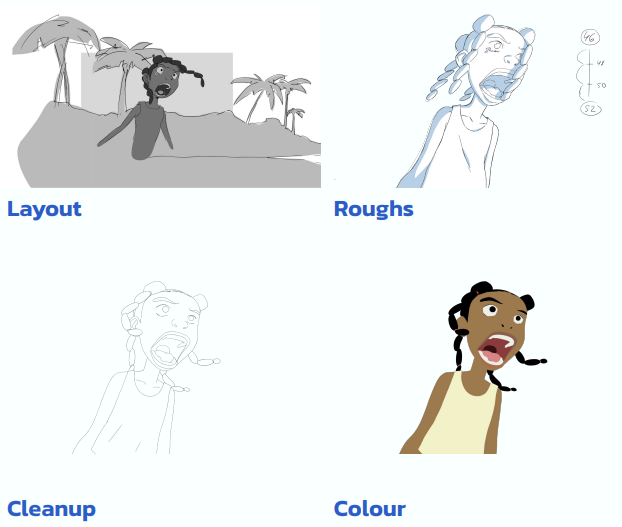
\includegraphics[width=0.75\textwidth]{images/introduction/stages.png}
    \caption{Sample frame for 4 stages of the workflow, including Layout, Roughs, Cleanup and Color.} 
    \label{fig:stages}
\end{figure}

Currently, lead artist gives front-loaded creative input followed by labor intensive tasks that he has little control. We want lead artist to get an accurate preview of what might be the final product. In particular, when they create the basis for character movement. We plan to create tools that enhance and speed up the process of creating 2D animation. The 2D animator will be offered more creative options in both movement and styles.

\subsubsection{Proposed System}

\begin{figure}
    \centering
    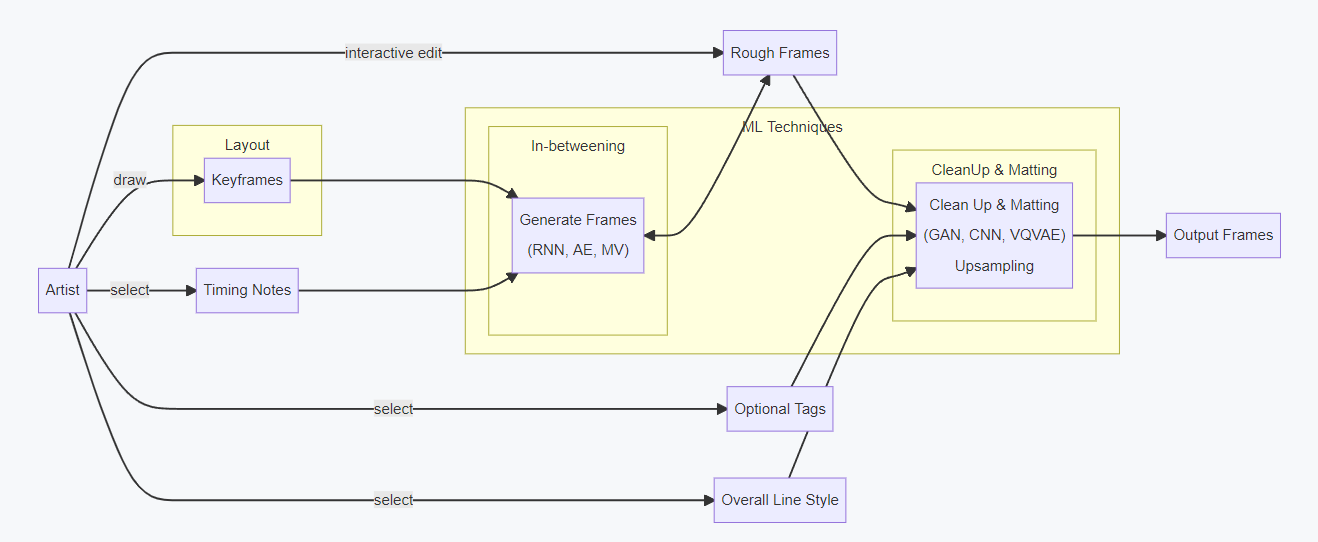
\includegraphics[width=1\textwidth]{images/introduction/proposed_workflow.png}
    \caption{Overview of proposed final workflow for the artist. The artist will produce a number of rough frames, with timing and style information. They will be feed into multiple machine learning (ML) pipelines to generate a preview of the final animation.} 
    \label{fig:proposed_worflow}
\end{figure}

In the proposed system, the artist will produce a number of rough keyframes with timing and styles information. These frames will go through 4 ML pipelines, each with different purposes: (1) clean up the rough sketches; (2) coloring; (3) frame interpolation (increase fps) and (4) upscaling (super resolution). Each method will be researched and a prototype model will be developed for proof-of-concept thesis (which is this thesis).


\section{General Approach}
\subsection{Image-to-Image Translation}
As you may have observed, all four tasks falls into the field of Image-to-Image translation (I2I), which is a sub-field in Computer Vision. I2I refers to the task of transforming images from one domain to another, so that they have the styles or characteristics from another domain. It has been gaining popularity in recent year due to its wide range of applications in computer vision problems such as image restoration, super resolution, segmentation and pose estimation. The scope of this project falls into two-domain, supervised I2I\cite{pangImagetoImageTranslationMethods2021}. Most recent research on I2I uses deep convolutional neural network to learn a mapping function between and source and target domain. Pix2pix\cite{isolaImagetoImageTranslationConditional2018} first successfully apply deep convolutional conditional GAN to solve a wide range of I2I problems. However, Pix2pix itself suffers from a number of issues. For example, it often produce blurry result due to use of L2 loss which minimizes the average loss\cite{wangDiscriminativeRegionProposal2018}; training might be unstable and error-prone as resolution increases\cite{wangHighResolutionImageSynthesis2018}; and unable to capture complex scene structure\cite{tangMultiChannelAttentionSelection2019}. Thus we will not directly apply it in our tasks, however, most models are either inspired by or follow the same architecture as Pix2pix.

%Pretraining + finetuning + feature content loss + WGAN-GP, cGAN + U-Net
\section{Evaluation Methods}
%mostly by eye, we can compute the PSNR and SSIM, but, generally eye is enough.
%Some stuff about things.\cite{example-citation} Some more things. 

%Inline citation: \bibentry{example-citation}

% This just dumps some pseudolatin in so you can see some text in place.
%\blindtext
